\documentclass[11pt]{beamer}
\usetheme{Pittsburgh}
\usepackage{xcolor}
\usepackage{pifont,enumitem}
\usepackage{etoolbox}
\usepackage{textpos}
\usepackage{capt-of}% or use the larger `caption` package
%\usepackage[pass]{geometry} 
\usepackage{multirow}
\usepackage{hhline} 
\usepackage{colortbl}
\usepackage{tikz}
\usetikzlibrary{trees,automata,positioning}
\usepackage{verbatim}
\usepackage{mathdots}
\usepackage{subcaption}

\setbeamertemplate{frametitle}{%
    \nointerlineskip%
    \usebeamerfont{frametitle}%
    \begin{beamercolorbox}[wd=\paperwidth,ht=1cm,sep=3pt]{frametitle}

        \includegraphics[height=1.2\baselineskip]{"VOUW logo-03"}
        \hfill\usebeamerfont{frametitle}\insertframetitle%

    \end{beamercolorbox}
}

\setbeamercolor{frametitle}{fg=red!45!yellow,bg=teal!75}
\setbeamercolor*{title}{fg=teal!75}
\usepackage{microtype}
\usepackage[utf8]{inputenc}

% import from STIX
\DeclareFontEncoding{LS1}{}{}
\DeclareFontSubstitution{LS1}{stix}{m}{n}
\DeclareFontFamily{LS1}{stixfrak}{\skewchar\font127 }
\DeclareFontShape{LS1}{stixfrak}{m}{n} {<-> stix-mathfrak}{}
\newcommand{\tplus}{\text{\usefont{LS1}{stixfrak}{m}{n}\symbol{"EB}}}
\newcommand{\tminus}{\text{\usefont{LS1}{stixfrak}{m}{n}\symbol{"EC}}}
%%%

\usepackage{amsmath}
\usepackage{amsfonts}
\usepackage{amssymb}
\usepackage{graphicx}
\usepackage[T1]{fontenc}
\usepackage{lmodern}
\usepackage{MnSymbol}

\setlist[itemize]{label={\color{red!45!yellow}\Pifont{pzd}{\char93}}}
\renewcommand{\mark}[1]{\textcolor{red!45!yellow}{\textbf{#1}}}
\renewcommand{\bold}[1]{\textcolor{teal}{\textbf{#1}}}

% Set the overall layout of the tree
\tikzstyle{level 1}=[level distance=4.0cm, sibling distance=.7cm]
\tikzstyle{level 2}=[level distance=4.5cm, sibling distance=.7cm]
\tikzstyle{level 3}=[level distance=3.5cm, sibling distance=.7cm]

% Define styles for bags and leafs
\tikzstyle{l1} = [rectangle, text width=5.5em]
\tikzstyle{l2} = [rectangle, text width=7em]
\tikzstyle{l3} = [rectangle, text width=5em, text centered]

\author{Micky Faas and Matthijs van Leeuwen}
\title{Geometric Pattern Mining using the MDL Principle}
%\setbeamercovered{transparent} 
%\setbeamertemplate{navigation symbols}{} 
%\logo{} 
\institute{LIACS, Leiden University, Leiden, the Netherlands} 
%\date{} 
%\subject{} 

\begin{document}
\beamertemplatenavigationsymbolsempty
\begin{frame}
\nointerlineskip%
\begin{columns}
\column{\dimexpr\paperwidth}
\centering % Center table

%%
%% Afbeelding 'triangles'
%% 
%% 32x32 = 1024 elements
%% geel = 8x3 elements
%% rood = 8x6 elements
%% blauw = 6x9 elements
%% groen = 3x12 elements
%% totaal = 25 patterns, 162 elements, 30 'pattern elements'
%%


\includegraphics[width=0.4\paperwidth]{"VOUW logo-02"} 
\maketitle
\end{columns}
\end{frame}

% Full image slide
\begin{frame}{Introduction}
\nointerlineskip%
\begin{columns}
\column{\dimexpr\paperwidth}
\centering
\includegraphics[scale=.3]{"triangles"} 
\end{columns}
\end{frame}

%%%%%%%%%%

% Full image slide
\begin{frame}{Example Matrix}
\nointerlineskip%
\begin{columns}
\column{\dimexpr\paperwidth}
\centering
\includegraphics[scale=.3]{"triangles_color"} 
\end{columns}
\end{frame}

%%%%%%%%%%

% Full image slide
\begin{frame}{`Compressed' Matrix}
\nointerlineskip%
\begin{columns}
\column{\dimexpr\paperwidth}
\centering
\includegraphics[scale=.3]{"triangles_compressed"} 
\end{columns}
\end{frame}

%%%%%%%%%%

\begin{frame}{Minimum Description Length}
\end{frame}

%%%%%%%%%%

\begin{frame}{Two-part MDL}

Idea: the best solution is a balance of model and instantiation complexity, given by:

$$
\underbrace{L(H)}_{\textsf{Model}} + \underbrace{L(A|H)}_{\textsf{Data given model}}
$$

In this case:

\begin{align*}
L\left(
\underbrace{
X=\overbrace{
\begin{bmatrix}
1 & \cdot \\[-.2em]
\cdot & 1
\end{bmatrix}}^{\textsf{Pattern}},
Y=\overbrace{
\begin{bmatrix}
1
\end{bmatrix}}^{\textsf{Pattern}}
}_{\textsf{Model}}
\right)
+
L\left(
\underbrace{ 
\overbrace{
\begin{matrix}
X & \cdot & \cdot & \cdot & \cdot & Y  \\[-.2em]
\cdot & \cdot & \cdot & \cdot & \cdot & \cdot  \\[-.2em]
X & \cdot & \cdot & \cdot & X & \cdot  \\[-.2em]
\cdot & \cdot & \cdot & \cdot & \cdot & \cdot  \\[-.2em]
X & \cdot & X & \cdot & \cdot & \cdot  \\[-.2em]
\cdot & \cdot & \cdot & \cdot & \cdot & \cdot  \\
\end{matrix}}}^{\textsf{Instantiation Matrix}}_{\textsf{Data given model}}
\right)
\end{align*}
\end{frame}

%%%%%%%%%%%%%

% Full image slide
\begin{frame}{Model and Instantiation Matrix}
\nointerlineskip%
\begin{columns}
\column{\dimexpr\paperwidth}
\centering
\includegraphics[scale=.3]{"triangles_compressed2"} 
\end{columns}
\end{frame}

%%%%%%%%%%

% Full image slide
\begin{frame}{Underfit Solution}
\nointerlineskip%
\begin{columns}
\column{\dimexpr\paperwidth}
\centering
\includegraphics[scale=.3]{"triangles_underfit"} 
\end{columns}
\end{frame}

%%%%%%%%%%

% Full image slide
\begin{frame}{Overfit Solution}
\nointerlineskip%
\begin{columns}
\column{\dimexpr\paperwidth}
\centering
\includegraphics[scale=.3]{"triangles_overfit"} 
\end{columns}
\end{frame}

%%%%%%%%%%%

\begin{frame}{Search Space Lattice}
\nointerlineskip%
\begin{columns}
\column{\dimexpr\paperwidth}
\centering
\includegraphics[scale=.25]{"lattice"} 
\end{columns}
\small Model space lattice for a 2 × 2 Boolean matrix. The V, W, and Z columns show which pattern is added in each step, while I depicts the current instantiation.
\end{frame}

%%%%%%%%%%%%%

\begin{frame}{Candidates}

\small Candidates are generated by enumerating all combinations of two adjacent patterns that occur in the instantiation matrix.\\ \medskip

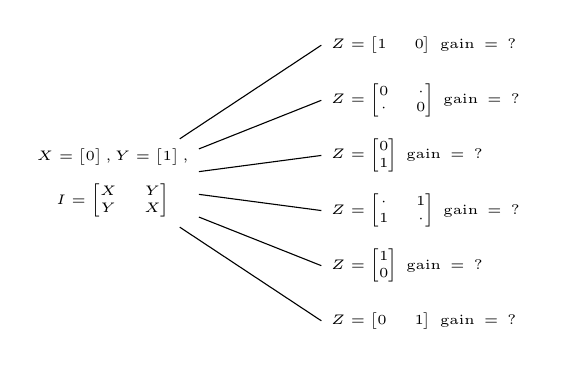
\begin{tikzpicture}[on grid, grow=right]
\node(R)[l1] {\tiny $\begin{matrix}X=\begin{bmatrix}0\end{bmatrix},Y=\begin{bmatrix}1\end{bmatrix},\\[1em]I=\begin{bmatrix}X & Y \\Y & X\end{bmatrix}\end{matrix}$}
	child {
        node(F)[l2] {\tiny $Z=\begin{bmatrix}0 & 1\end{bmatrix}$ gain = ?}        
            edge from parent[draw=none] 
            (R) edge (F.west)
    }
    child {
        node(E)[l2] {\tiny $Z=\begin{bmatrix}1 \\ 0\end{bmatrix}$ gain = ?}        
            edge from parent[draw=none] 
            (R) edge (E.west)
    }    
    child {
        node(D)[l2] {\tiny $Z=\begin{bmatrix}\cdot & 1 \\ 1 & \cdot\end{bmatrix}$ gain = ?}        
            edge from parent[draw=none] 
            (R) edge (D.west)
    }    
    child {
        node(C)[l2] {\tiny $Z=\begin{bmatrix}0 \\ 1\end{bmatrix}$ gain = ?}              
            edge from parent[draw=none] 
            (R) edge (C.west)
    }    
    child {
        node(B)[l2] {\tiny $Z=\begin{bmatrix}0 & \cdot \\ \cdot & 0\end{bmatrix}$ gain = ?}               
            edge from parent[draw=none] 
            (R) edge (B.west)
    } 
    child {
        node(A)[l2] {\tiny $Z=\begin{bmatrix}1 &0\end{bmatrix}$ gain = ?}        
        	edge from parent[draw=none] 
            (R) edge (A.west)
    };
\end{tikzpicture}
\end{frame}

%%%%%%%%%%%

\begin{frame}{Length and Gain}

$$
	\underbrace{\Delta L(A',c)}_{\textsf{Gain}} = \underbrace{\Big(L_1(H') + L_2(I') \Big)}_{\textsf{New Lengths}} - \underbrace{\Big(L_1(H) + L_2(I) \Big)}_{\textsf{Old Lengths}}
$$

\small $L_1$ and $L_2$ are independent length functions that compute the length of the model and the instantiation, respectively. \\ \medskip
\emph{Please see the paper for more information on the encoding scheme.}


\end{frame}


%%%%%%%%%%

\begin{frame}{Pattern Union}
We can construct complex patterns by repeatedly combining simpler ones. We use instances for this as they encode the position of one pattern relative to another.

\begin{align*}
\underbrace{
\begin{matrix}
X = \begin{bmatrix}
0
\end{bmatrix} \\[1.0em]
Y = \begin{bmatrix}
1
\end{bmatrix}
\end{matrix}}_{\textsf{Candidate patterns}}
\longrightarrow
\underbrace{\begin{matrix}
\bar{X} = \begin{bmatrix}
\cdot  & \cdot & \cdot \\
0 & \cdot & \cdot \\
\cdot & \cdot & \cdot \\
\end{bmatrix} \\[1.0em]
\bar{Y} = \begin{bmatrix}
\cdot  & \cdot & \cdot \\
\cdot  & \cdot & \cdot \\
\cdot & 1 & \cdot
\end{bmatrix}
\end{matrix}}_{\textsf{Instances}}
\longrightarrow
\bar{X}+\bar{Y} =
\underbrace{
\begin{bmatrix}
\cdot  & \cdot & \cdot \\
0  & \cdot & \cdot \\
\cdot & 1 & \cdot
\end{bmatrix}}_{\textsf{Matrix sum}}
\longrightarrow
\underbrace{
\begin{bmatrix}
0  & \cdot \\
\cdot & 1 
\end{bmatrix}}_{\textsf{New pattern}}
\end{align*}
\end{frame}


%%%%%%%%%%%%%

\begin{frame}{Simplified Algorithm}

\tikzset{every picture/.style={line width=0.75pt}} %set default line width to 0.75pt        

\tiny
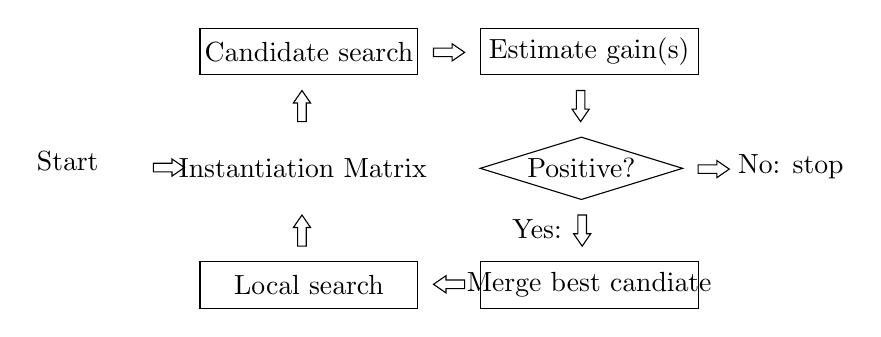
\begin{tikzpicture}[x=0.75pt,y=0.75pt,yscale=-.75,xscale=.75]
%uncomment if require: \path (0,300); %set diagram left start at 0, and has height of 300

%Flowchart: Process [id:dp4782497477496759] 
\draw   (200,60) -- (340,60) -- (340,90) -- (200,90) -- cycle ;
%Right Arrow [id:dp0106127781483073] 
\draw   (350,72.75) -- (362,72.75) -- (362,70) -- (370,75.5) -- (362,81) -- (362,78.25) -- (350,78.25) -- cycle ;
%Flowchart: Process [id:dp8391634624078887] 
\draw   (380,60) -- (520,60) -- (520,90) -- (380,90) -- cycle ;
%Right Arrow [id:dp2784645145213487] 
\draw   (447.25,100) -- (447.25,112) -- (450,112) -- (444.5,120) -- (439,112) -- (441.75,112) -- (441.75,100) -- cycle ;
%Flowchart: Process [id:dp41447896123303685] 
\draw   (380,210) -- (520,210) -- (520,240) -- (380,240) -- cycle ;
%Flowchart: Decision [id:dp26196178425216665] 
\draw   (445,130) -- (510,150) -- (445,170) -- (380,150) -- cycle ;
%Right Arrow [id:dp7826103447038623] 
\draw   (448.25,180) -- (448.25,192) -- (451,192) -- (445.5,200) -- (440,192) -- (442.75,192) -- (442.75,180) -- cycle ;
%Right Arrow [id:dp5430390369649105] 
\draw   (520,147.75) -- (532,147.75) -- (532,145) -- (540,150.5) -- (532,156) -- (532,153.25) -- (520,153.25) -- cycle ;
%Flowchart: Process [id:dp3531450147225088] 
\draw   (200,210) -- (340,210) -- (340,240) -- (200,240) -- cycle ;
%Right Arrow [id:dp5376430472123639] 
\draw   (262.75,200) -- (262.75,188) -- (260,188) -- (265.5,180) -- (271,188) -- (268.25,188) -- (268.25,200) -- cycle ;
%Right Arrow [id:dp8138585643184836] 
\draw   (262.75,120) -- (262.75,108) -- (260,108) -- (265.5,100) -- (271,108) -- (268.25,108) -- (268.25,120) -- cycle ;
%Right Arrow [id:dp9102501544724863] 
\draw   (170,152.25) -- (182,152.25) -- (182,155) -- (190,149.5) -- (182,144) -- (182,146.75) -- (170,146.75) -- cycle ;
%Flowchart: Process [id:dp10502859111005758] 
%\draw   (70,130) -- (160,130) -- (160,160) -- (70,160) -- cycle ;
%Right Arrow [id:dp67324525964606] 
\draw   (370,227.25) -- (358,227.25) -- (358,230) -- (350,224.5) -- (358,219) -- (358,221.75) -- (370,221.75) -- cycle ;

% Text Node
\draw (270,75) node  [align=left] {Candidate search};
\draw (450,75) node  [align=left] {Estimate gain(s)};
\draw (450,225) node  [align=left] {Merge best candiate};
\draw (445,150) node  [align=left] {Positive?};
\draw (579.5,149) node  [align=left] {No: stop};
\draw (416.5,189) node  [align=left] {Yes:};
\draw (270,225) node  [align=left] {Local search};
\draw (266,150) node  [align=left] {Instantiation Matrix};
%\draw (243.5,111) node  [align=left] {No:};
\draw (115,145) node  [align=left] {Start};
%\draw (183.5,131) node  [align=left] {Yes:};
\end{tikzpicture}
\end{frame}

%%%%%%%%%%

% Full image slide
\begin{frame}{Experiments}
\nointerlineskip%


\begin{figure}[t]
\centering
\begin{subfigure}[t]{0.25\textwidth}
\centering
\includegraphics[scale=.8]{exp_input_2.png}
\caption{Generated matrix}
\label{fig:rila}
\end{subfigure}%
~
\begin{subfigure}[t]{0.25\textwidth}
\centering
\includegraphics[scale=.8]{exp_inputpatterns_2.png}
\caption{Ground truth}
\label{fig:rilb}
\end{subfigure}%
~
\begin{subfigure}[t]{0.25\textwidth}
\centering
\includegraphics[scale=.8]{exp_result_2.png}
\caption{Found patterns}
\label{fig:rilc}
\end{subfigure}%
~
\begin{subfigure}[t]{0.25\textwidth}
\centering
\includegraphics[scale=.8]{exp_diff_2.png}
\caption{Difference}
\label{fig:rild}
\end{subfigure}%
\caption{Synthetic patterns are added to a matrix filled with noise. The difference between the ground truth and the matrix reconstructed by the algorithm is used to compute precision and recall.}
\label{fig:ril}
\end{figure}  

\end{frame}

%%%%%%%%%%%

% Full image slide
\begin{frame}{Compression and SNR}
\nointerlineskip%
\begin{columns}
\column{\dimexpr\paperwidth}
\centering
\includegraphics[scale=1]{"results_compression"} 
\end{columns}
\bigskip
\small Results for different square matrices ($256 \times 256$ to $1024 \times 1024$). Signal-to-noise ratio is computed as $\frac{\textsf{signal}}{\textsf{signal}+\textsf{noise}}$.

\end{frame}

%%%%%%%%%%%

\begin{frame}{\large: Geometric Pattern Mining using the MDL principle}

\small
The article was published at the Symposium on Intelligent Data Analysis (IDA) 2020\\ \smallskip
Archive link: \texttt{\textcolor{blue}{http://arxiv.org/abs/1911.09587}}\\ \smallskip
Code repository: \texttt{\textcolor{blue}{https://github.com/mickymuis/libvouw}}\\ \smallskip
Contact the authors:\\ \smallskip
Micky Faas \texttt{\textcolor{blue}{<micky@edukitty.org>}}\\ \smallskip
Matthijs van Leeuwen \texttt{\textcolor{blue}{<m.van.leeuwen@liacs.leidenuniv.nl>}}\\ \bigskip
\emph{Thank you for watching!}



\end{frame}

\end{document}